\documentclass[10pt,a4paper]{article}
\usepackage[utf8]{inputenc}
\usepackage{amsmath}
\usepackage{amsfonts}
\usepackage{amssymb}
\usepackage{amsthm}
\usepackage{amsbsy}
\usepackage[
  margin=1.5cm,
  includefoot,
  footskip=30pt,
]{geometry}
\usepackage{layout}
\usepackage{graphicx}
\usepackage{listings}
\lstset{frame=tb,
  language=Python,
}
\author{Raphaël Avalos}
\title{Reinforcement Learnig: Homework 2}
\begin{document}
\maketitle

\section{Question 1}
The following two Bernouili Bandit problem cosnidered are represented in the table bellow. The following plots are an average of $1000$ simulations with $\rho = 0.2$.\\


\begin{tabular}{|c|c|c|c|c|}
\hline 
 & Arm 0 & Arm 1 & Arm 2 & Arm 3 \\ 
\hline 
First Problem $p=$ & 0.65 & 0.5 & 0.45 & 0.6 \\ 
\hline 
Second Problem $p=$ & 0.43 & 0.56 & 0.51 & 0.55 \\ 
\hline 
\end{tabular} 
\\

\begin{figure}[h]
\centering
\begin{minipage}{0,45\textwidth}
\caption{MAB 1}
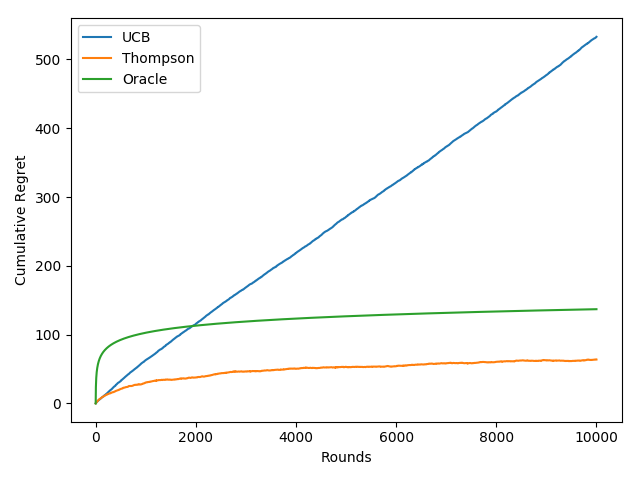
\includegraphics[scale=.45]{mab_1.png}
\end{minipage}
\begin{minipage}{0,45\textwidth}
\caption{MAB 2}
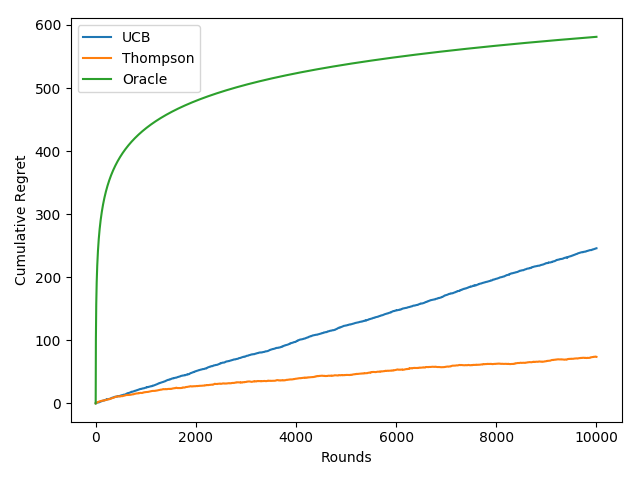
\includegraphics[scale=.45]{mab_2.png}
\end{minipage}
\end{figure}
\newpage
\section{Question 2}

The Thomson algorithm has been adapted in the following way.
\begin{lstlisting}
arm = np.random.beta(S + 1, F + 1).argmax()
reward = bandits[arm].sample()
draws[t] = arm
N[arm] += 1
    if np.random.random() < reward:
        S[arm] += 1
    else:
        F[arm] += 1
\end{lstlisting}

\begin{tabular}{|c|c|c|c|c|}
\hline 
 & Arm 0 & Arm 1 & Arm 2 & Arm 3 \\ 
\hline 
Parameters & $\mathcal{B}(0.7,0.6)$ & $\mathcal{B}(0.5,0.6)$ & $\mathbf{Exp}(0.7)$ & $\mathbf{Exp}(0.35)$ \\ 
\hline 
\end{tabular} 
\\
\begin{figure}[h]
\centering
\begin{minipage}{0,45\textwidth}
\caption{NPM}
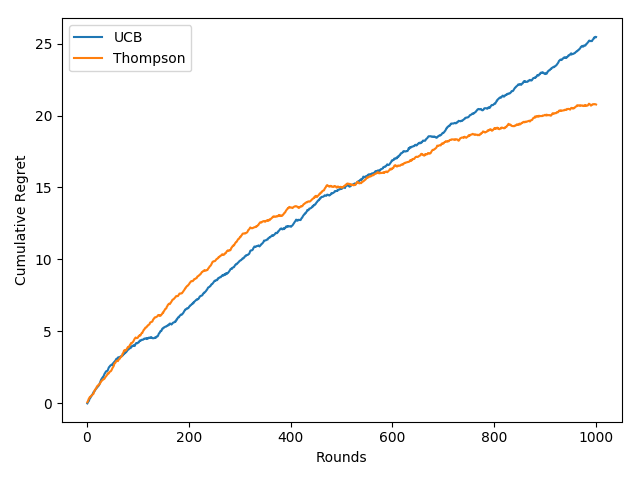
\includegraphics[scale=.45]{npm.png}
\end{minipage}
\end{figure}
\newpage
\section{Question 3}
In LinearUCB the parameter $\alpha$ affects the exploration. I choose $\alpha_0 = 100$ and $\alpha_{t+1} = max(0,\alpha_t - 1)$ and $\lambda = 1$. The plots are the average over 30 runs with 6000 epochs.\\
LinearUCB provides the minimal cummulative regret by sacrifacing exploration thereore it doen't compute a great approximation of $\theta$.

\begin{figure}[h]
\centering
\begin{minipage}{0,90\textwidth}
\caption{LineraUCB vs Random vs Greedy}
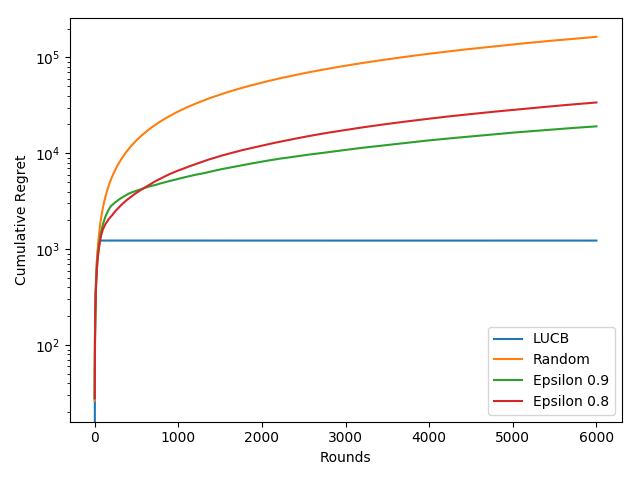
\includegraphics[scale=.40]{q3_1.png}
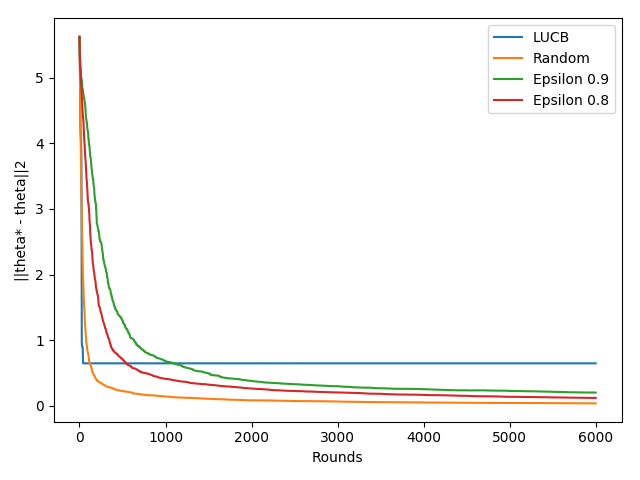
\includegraphics[scale=.40]{q3_2.png}
\end{minipage}
\end{figure}

\end{document}